% !TEX program = xelatex
\documentclass{article}
\usepackage{ctex}
\usepackage{fontawesome}
\usepackage{tikz}
\usetikzlibrary{arrows,decorations.markings}
\usetikzlibrary{decorations.pathreplacing}
\usetikzlibrary{calc}

\begin{document}
\begin{tikzpicture}[decoration={
    markings,
    mark=at position 1 with {\arrow[scale=1]{angle 90}};
  }]
  \draw [decorate,decoration={brace,amplitude=10pt,mirror}]
(-0.1,-1) --node [black,midway,below,sloped,yshift=-10pt] {建立连接}  (-0.1,-7.2);
\draw [decorate,decoration={brace,amplitude=10pt,mirror},color=blue]
(-0.1,-7.5) --node [black,midway,below,sloped,yshift=-10pt,xshift=-1cm,color=blue] {发送数据}  (-0.1,-12);

  \draw[->,dashed,line width=2,color=gray] (0,-0.5) node[above,color=black]{\large{$A$}} -- (0,-9);
  \draw[->,dashed,line width=2,color=gray] (8,-0.5) node[above,color=black]{\large{$B$}} -- (8,-9);
  \draw[->,line width=1,postaction={decorate}] (0,-1) --node[above,sloped]{\texttt{SYN=1, seq=0}} (8,-3);
  \draw[->,line width=1,postaction={decorate}] (8,-3.1) --node[above,sloped]{\texttt{SYN=1, seq=0, ack=1}} (0,-5.1);
  \draw[->,line width=1,postaction={decorate}] (0,-5.2) --node[above,sloped]{\texttt{{\textcolor{gray}{SYN=0, }
  }seq=1, ack=1}} (8,-7.2);
%  \draw[->,line width=1,postaction={decorate}] (0,-7.5) --node[above,sloped]{\texttt{seq=2, 500B数据}} (8,-9.5);
%  \draw[->,line width=1,postaction={decorate}] (8,-9.7) --node[above,sloped]{\texttt{ACK=1, ack=502}} (0,-11.7);


\end{tikzpicture}

\begin{tikzpicture}[decoration={
    markings,
    mark=at position 1 with {\arrow[scale=1]{angle 90}};
  }]
  
  \draw[->,dashed,line width=2,color=gray] (0,-0.5) node[above,color=black]{\large{$A$}} -- (0,-17.5);
  \draw[->,dashed,line width=2,color=gray] (8,-0.5) node[above,color=black]{\large{$B$}} -- (8,-17.5);
  {\scriptsize
  \draw<1->[->,line width=1,color=blue,postaction={decorate}] (0,-1) --node[above,sloped,pos=0.25]{\texttt{seq=1, 500B数据}} (8,-3);
  \draw<2->[->,line width=1,postaction={decorate}] (8,-3.1) --node[above,sloped,pos=0.25]{\texttt{ack=501,\textcolor{gray}{seq=1}}} (0,-5.1);
  \draw<3->[->,line width=1,color=red,postaction={decorate}] (0,-2) --node[above,sloped,pos=0.333]{\texttt{seq=501, 500B数据}} (6,-3.5) node[right]{\large{\faClose}};
  \draw<4->[->,line width=1,color=blue,postaction={decorate}] (0,-3) --node[above,sloped,pos=0.25]{\texttt{seq=1001, 500B数据}} (8,-5);
  \draw<5->[->,line width=1,color=blue,postaction={decorate}] (0,-4) --node[above,sloped,pos=0.25]{\texttt{seq=1501, 500B数据}} (8,-6);
  \draw<5->[->,line width=1,postaction={decorate}] (8,-5.1) --node[above,sloped,pos=0.25]{\texttt{ack=1501,\textcolor{gray}{seq=1}}} (0,-7.1);
  \draw<6->[->,line width=1,postaction={decorate}] (8,-6.1) --node[above,sloped,pos=0.25]{\texttt{ack=2001,\textcolor{gray}{seq=1}}} (0,-8.1);
  \draw<7->[->,line width=1,color=red,postaction={decorate}] (0,-8.5) --node[above,sloped,pos=0.333]{\texttt{seq=501, 500B数据}} (6,-10) node[right]{\large{\faClose}};
  \draw<8->[->,line width=1,color=blue,postaction={decorate}] (0,-10.5) --node[above,sloped,pos=0.25]{\texttt{seq=501, 500B数据}} (8,-12.5);
  \draw<9->[->,line width=1,postaction={decorate}] (8,-12.6) --node[above,sloped,pos=0.25]{\texttt{ack=1001,\textcolor{gray}{seq=1}}} (0,-14.6);
  \draw<10->[->,line width=1,color=blue,postaction={decorate}] (0,-14.8) --node[above,sloped,pos=0.25]{\texttt{seq=2001, 500B数据}} (8,-16.8);
  \draw<10-> (4, -16.5) node {$\vdots$};
}

\end{tikzpicture}

\vspace{1cm}

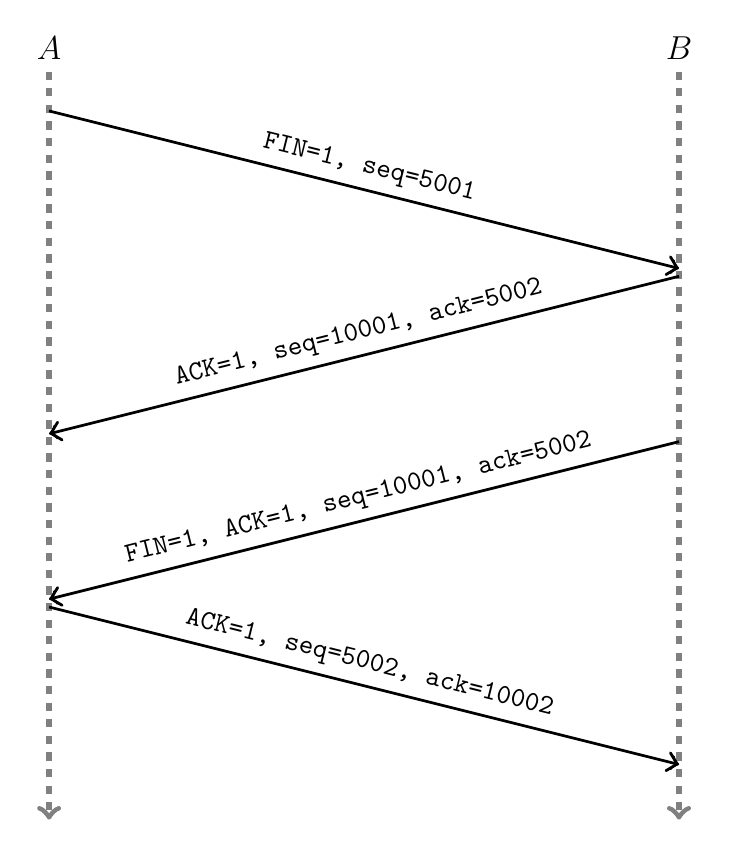
\begin{tikzpicture}[decoration={
      markings,
      mark=at position 1 with {\arrow[scale=1]{angle 90}};
  }]
\draw[->,dashed,line width=2,color=gray] (0,-0.5) node[above,color=black]{\large{$A$}} -- (0,-10);
\draw[->,dashed,line width=2,color=gray] (8,-0.5) node[above,color=black]{\large{$B$}} -- (8,-10);
\draw[->,line width=1,postaction={decorate}] (0,-1) --node[above,sloped]{\texttt{FIN=1, seq=5001}} (8,-3);
\draw[->,line width=1,postaction={decorate}] (8,-3.1) --node[above,sloped]{\texttt{ACK=1, seq=10001, ack=5002}} (0,-5.1);
\draw[->,line width=1,postaction={decorate}] (8,-5.2) --node[above,sloped]{\texttt{FIN=1, ACK=1, seq=10001, ack=5002}} (0,-7.2);
\draw[->,line width=1,postaction={decorate}] (0,-7.3) --node[above,sloped]{\texttt{ACK=1, seq=5002, ack=10002}} (8,-9.3);

\end{tikzpicture}
\end{document}
